\documentclass[11pt]{article}
\usepackage[utf8]{inputenc}
\usepackage{graphicx}
\usepackage{geometry}
\usepackage{parskip}
\usepackage{subcaption}
\usepackage{wrapfig}
\usepackage{acronym}
\usepackage[natbib=true]{biblatex}
\usepackage{amsmath}
\usepackage{csquotes}
\usepackage{hyperref}
\addbibresource{literature.bib}
\renewcommand{\baselinestretch}{1.5}
\newcounter{savepage}

\begin{document}

    \begin{titlepage}
        \centering
        
\includegraphics[width=0.25\textwidth]{rublogo.png}\par
        {\scshape\huge\bfseries Semantic Representations in Variational Autoencoders as a Model of the Visual System \par}
        {\scshape\large Schriftliche Prüfungsarbeit für die Master-Prüfung des Studiengangs Angewandte Informatik an der Ruhr-Universität Bochum\par}
        \vspace{1em}
        vorgelegt von\par
        \vspace{2em}
        Leonard Papenmeier\par 108017257755\par
        \vspace{2em}
        01.01.1980\par

        \vfill
        Prof. Dr. Laurenz Wiskott\par
        M.Sc. Zahra Fayyaz


    \end{titlepage}
    \pagenumbering{Roman}
    \tableofcontents
    \newpage
    \setcounter{savepage}{\arabic{page}}
    \pagenumbering{arabic}

    \section{Introduction}\label{sec:introduction}
    \section{Theoretical Background}\label{sec:theoretical-background}
    \subsection{Primary Visual Cortex}\label{subsec:primary-visual-cortex}
    \subsection{Variational Autoencoders}\label{subsec:variational-autoencoders}
    \subsection{Visual Features in Neural Networks}\label{subsec:visual_features_in_neural_networks}
    \begin{itemize}
        \item~\cite{krizhevsky2012imagenet} report Gabor wavelets in \acp{CNN} trained on image classification
    \end{itemize}
    \subsection{Semantic Representations}\label{subsec:semantic-representations}
    \subsubsection{Supervised Models}
    \begin{itemize}
        \item \citet{khaligh2014deep} found evidence for that supervised models may explain \ac{IT} cortical representation.
    \end{itemize}

    \subsubsection{Unsupervised Models}
    \begin{itemize}
        \item \citet{han2019variational} found no evidence for or against Gabor wavelets in \acp{VAE} due to too small kernel size
        \item \citet{khaligh2014deep} found evidence against the assumption that unsupervised models might explain \ac{IT} cortical representation, however not explicitly for \acp{VAE}
    \end{itemize}


    \section{Methods}\label{sec:methods}
    The following Sections describe the methods used in the course of this thesis.

\subsection{Implementation Details}\label{subsec:implementation-details}

All models are implemented with Keras\footnote{\href{https://keras.io/}{https://keras.io/}, last access: 07/01/2020} in Version 2.2.4 using the TensorFlow\footnote{\href{https://www.tensorflow.org/}{https://www.tensorflow.org/}, last access: 07/01/2020} backend in Version 1.15..
The models are trained on Tesla V100-DGXS GPUs with 16GB of RAM.
The model code can be found under \href{https://github.com/LeoIV/master-thesis-leonard}{https://github.com/LeoIV/master-thesis-leonard}.

\subsection{Datasets}\label{subsec:datasets}

Five different datasets were used to train the models.
Four of the datasets contain images of different sizes, the fifth dataset provides additional labels for the \textsc{Mnist} dataset.
The images were resized to match the model's expected input sizes using Lanczos interpolation~\citep[pp. 223, ff]{burger2009principles}.

\subsubsection{CelebA}\label{subsubsec:celeba_dataset}

\begin{wrapfigure}[14]{R}{0.3\textwidth}
    \begin{center}
        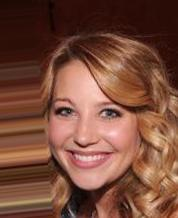
\includegraphics[width=0.28\textwidth]{images/celeba_sample_63.jpg}
    \end{center}
    \caption[CelebA dataset sample image]{A sample image from the CelebA dataset.}
    \label{fig:celeba_sample}
\end{wrapfigure}

The \textit{CelebA} dataset~\citep{liu2015faceattributes} consists of 202,599 RGB images of size 178 x 218 pixels representing celebrities, as well as 40 binary attributes.
The images belong to 10.177 unique identities\footnote{The identities are not revealed.} as well as five \say{landmark annotations}.
They are aligned and cropped resulting in images of same size always showing only one face (see Figure~\ref{fig:celeba_sample} for an example).
The landmark annotations give the positions of facial attributes in the image; the left and right eye, the nose, and the left and right corner of the mouth.
The binary attributes indicate if the image has certain characteristics, for example if the person wears eyeglasses, has black hair, is smiling\footnote{See \href{https://www.kaggle.com/jessicali9530/celeba-dataset\#list\_attr\_celeba.csv}{https://www.kaggle.com/jessicali9530/celeba-dataset\#list\_attr\_celeba.csv} for a complete list of the attributes, login required. Last access: 12/02/2020.}.

\subsubsection{ImageNet}\label{ssec:imagenet}

ImageNet\footnote{\href{http://image-net.org/}{http://image-net.org/}, last access: 12/02/2020.} is a large-scale \say{image database organized according to the WordNet hierarchy}~\citep{imagenet_cvpr09}.
It contains of over 14 million images as of February 2020.
According to WordNet\footnote{See \href{https://wordnet.princeton.edu/}{https://wordnet.princeton.edu/}, last access: 12/02/2020.}, the images are subdivided into groups called \say{synsets}~\citep{imagenet_cvpr09} on different levels of granularity.
For example, the group \textit{woman, adult female} is subordinated to \textit{person, individual, someone, somebody, mortal, soul} and is further subdivided into groups like \textit{old woman} or \textit{lady} \footnote{ImageNet 2011 Fall Release, \href{http://image-net.org/explore}{http://image-net.org/explore}, last access: 12/02/2020.}

A smaller version of ImageNet, commonly called \textit{ILSVRC2012} has been used for \ac{ILSVRC2017}~\citep{ILSVRC15}, consisting of approximately 1,3 million images from 1000 different classes, that were selected, such that \say{there is no overlap between synsets: for any synsets $i$ and $j$, $i$ is not an ancestor of $j$ in the ImageNet hierarchy}~\citep{imagenet_cvpr09}.

This curated version is commonly used as a baseline (\textbf{refs}).

\subsubsection{Mnist}\label{subsubsec:mnist}

\begin{wrapfigure}[9]{R}{0.2\textwidth}
    \begin{center}
        
\includegraphics[width=0.18\textwidth]{images/mnist_sample.png}
    \end{center}
    \caption[\textsc{Mnist} dataset sample image]{A sample image from the \textsc{Mnist} dataset.}
    \label{fig:mnist_sample}
\end{wrapfigure}

\textsc{Mnist}\footnote{\href{http://yann.lecun.com/exdb/mnist/}{http://yann.lecun.com/exdb/mnist/}, last access: 23/04/2020}~\citep{lecun1998gradient} is a widely-used dataset of hand-written digits.
The data is subdivided into a training set of 60.000 images and a test set containing 10.000 images.
The digits are all of the same size and centered.
The samples are grayscale images of size $28\times 28$pixels.

\subsubsection{Morpho-\textsc{Mnist}}\label{subsubsec:morphomnist}

\begin{figure}
    \centering
    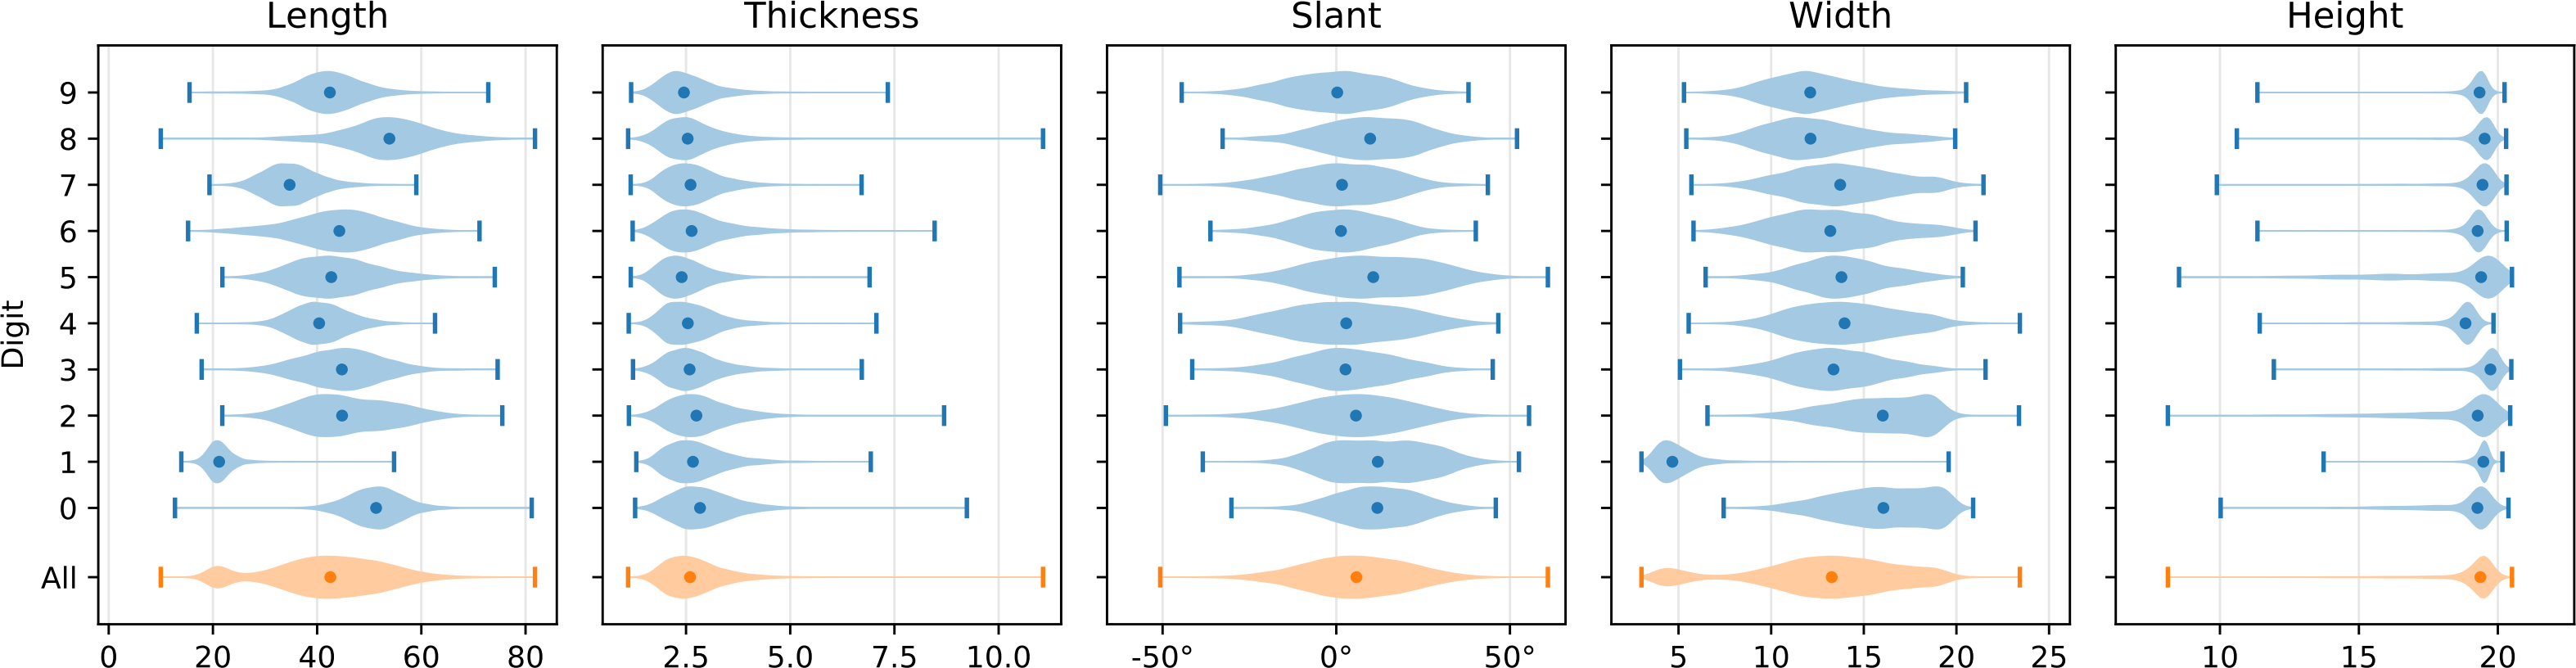
\includegraphics[width=\textwidth]{images/morpho_mnist_distribution.png}
    \caption[Morpho-\textsc{Mnist} distribution]{Distribution of the Morpho-\textsc{Mnist} attributes for the different digits. Taken from~\citep{castro2019morpho}.}
    \label{fig:morpho_mnist_distribution}
\end{figure}

Morpho-\textsc{Mnist}~\citep{castro2019morpho} is an extension of the \textsc{Mnist} dataset that addresses the question: \say{[T]o what extent has my model learned to represent specific factors of
variation in the data?} ~\citep{castro2019morpho}.
To address this questions, Morpho-\textsc{Mnist} provides the following (continuous) labels of morphological attributes of the \textsc{Mnist} samples: stroke length, stroke thickness, slant, width, and height.

Besides providing additional labels of low-level \textsc{Mnist} attributes, Morpho-\textsc{Mnist} provides a toolbox to measure (i.e~ calculate the morphological labels) and perturb MNIST images.
The perturbation toolbox allows it to thin, thicken, swell, and to add fractures to an image.
Morpho-\textsc{Mnist} also provides pre-computed datasets that were built using the perturbation toolbox.

Importantly, the distribution of the morphological attributes partly is highly skewed (for example Thickness and Height, see Figure~\ref{fig:morpho_mnist_distribution}).

\subsubsection{dSprites}
dSprites\footnote{\href{https://github.com/deepmind/dsprites-dataset/}{https://github.com/deepmind/dsprites-dataset/}, last access: 5/28/2020}~\citep{dsprites17} is a dataset designed \say{to assess the disentanglement properties of unsupervised learning methods.}.
It contains 737,280 grayscale images of size $64\times 64$ pixels.
The images were generated from \say{6 ground truth independent latent factors}: color, shape, scale, orientation, $x$-position, and $y$-position.
The color is white in all images.
The shapes are: square, ellipse, and heart.
For the other factors, points are chosen evenly along their support: six values in $[0.5, 1]$ (scale), 40 values in $[0, 2\pi]$ (orientation), 32 values in $[0, 1]$ ($x$-position and $y$-position).
Each factor combination only occurs once in the data set.
The dataset also contains the factor labels for each image.

\subsection{Models}\label{subsec:models}

Four different base \ac{VAE} models were evaluated in the course of this thesis.
Furthermore, two \say{AlexNet} models were used for some additional experiments.

The models vary depending on the dataset and are described in the following.
A more detailed description can be found in Appendix~\ref{sec:appendix_network_architectures}.

\subsubsection{VAE Models}\label{subsubsec:vae_models}

\begin{figure}
    \centering
    \begin{subfigure}{.5\textwidth}
        \centering
        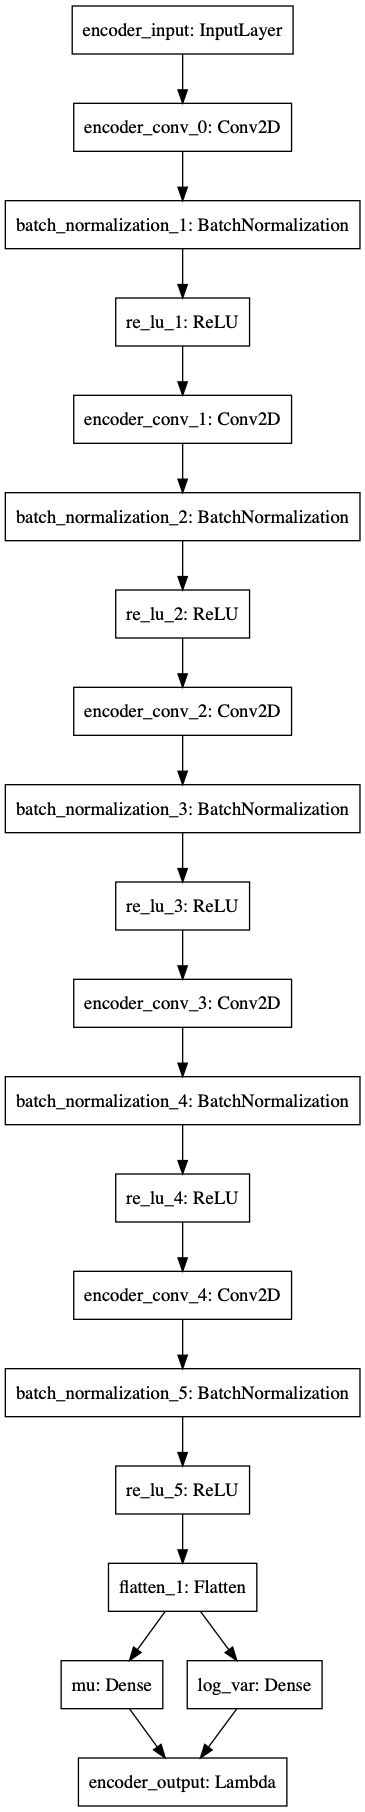
\includegraphics[width=\textwidth,height=.85\textheight,keepaspectratio]{images/vae/encoder.png}
        \caption{Encoder}
    \end{subfigure}%
    \begin{subfigure}{.5\textwidth}
        \centering
        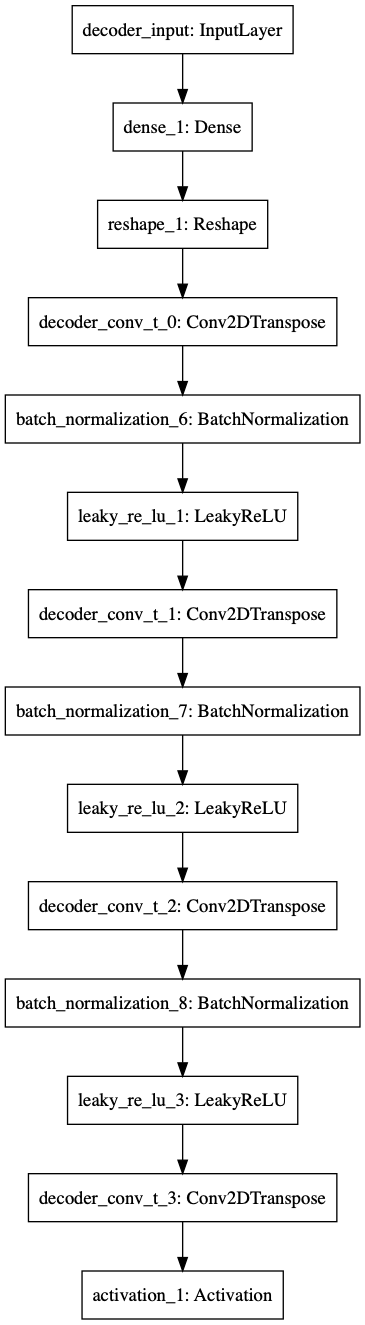
\includegraphics[width=\textwidth,height=.85\textheight,keepaspectratio]{images/vae/decoder.png}
        \caption{Decoder}
    \end{subfigure}
    \caption{\ac{VAE} model structure}
    \label{fig:vae_model_structure}
\end{figure}

The \ac{VAE} model (see Section-\ref{fig:vae_model_structure}) consists of an encoder and a decoder.
The encoder is made up of multiple \say{Convolution, Activation, Batch-Normalization}-blocks, followed by the embedding layer.
The embedding layer predicts $\mu$ and $\log \sigma^2$ and performs the resampling by:
\begin{align}
    z &= \mu + \epsilon\sigma \\
    \epsilon &\sim \mathcal{N}(0, \bm{I}). \label{eq:resampling_vae}
\end{align}
The encoder input size is equal to the decoder output size and is depending on the dataset.
The number of \say{Convolution, Activation, Batch-Normalization}-blocks is chosen depending on the input size, as smaller input sizes require fewer layers to achieve a receptive field of the input size.
The batch-normalization~~\citep[pp. 317, ff.]{Goodfellow-et-al-2016} can be omitted\footnote{It is stated in the experiments if batch-normalization is omitted.}.
The activation can be either ReLU~\citep[p. 173]{Goodfellow-et-al-2016} or LeakyReLU~\citep[p. 192]{Goodfellow-et-al-2016} and is ReLU unless stated otherwise.
The convolutions use zero-padding unless stated otherwise.
Encoder and decoder use stridden convolutions for downsampling, unless stated otherwise.

The \ac{VAE} model implements the loss function from Equation~\ref{eq:elbo_error_term} but with a pre-factor for the reconstruction term.
The reconstruction term pre-factor was determined empirically, observing reconstruction and generation quality.

The decoder uses similar blocks as the encoder but employs transposed convolutions~\citep[pp. 356, ff.]{Goodfellow-et-al-2016} instead of convolutions to upsample feature maps.
The output layer of the decoder uses a sigmoid activation instead of ReLU.

In total, eight \ac{VAE}-models are used: \say{\textsc{Mnist}-\ac{VAE}}, \say{dsprites-\ac{VAE}}, \say{7,500-\ac{VAE}}, \say{6,250-\ac{VAE}}, \say{5,000-\ac{VAE}},  \say{3,750-\ac{VAE}}, \say{dsprites-\ac{VAE}-dim6}, and \say{CelebA-\ac{VAE}}.
The model structures can be found in Appendix~\ref{subseq:appendix_vae_models}.

\paragraph{\textsc{Mnist}-\ac{VAE}} \textsc{Mnist}-\ac{VAE} uses an input- and output-size of $28\times 28\times 1$ (\textsc{Mnist} images are grayscale images).
The model is trained with the Adam optimizer on the \textsc{Mnist} training set with a batch size of 128 and a learning rate of 0.001 for 200 epochs.
The reconstruction loss factor is 10,000.
The latent space is two-dimensional.
The inner activation function is ReLU.

\paragraph{dSprites-\ac{VAE}} dSprites-\ac{VAE} uses an input- and output-size of $64\times 64\times 1$.
The model is trained with the Adam optimizer on a training set consisting of 90\% of the dSprites dataset with a batch size of 128 and a learning rate of 0.001 for 200 epochs.
The reconstruction loss factor is 10,000.
The latent space is ten-dimensional.
The inner activation function is ReLU.
For dSprites, four additional models have been trained with a different reconstruction term weight: 7,500-\ac{VAE}, 6,250-\ac{VAE}, 5,000-\ac{VAE}, and 3,750-\ac{VAE}.
These models differ from dSprites-\ac{VAE} only in the reconstruction term weight.

\paragraph{dsprites-\ac{VAE}-dim6}
The dsprites-\ac{VAE}-dim6 is equivalent to the dSprites-\ac{VAE} model but uses a six-dimensional latent space.

\paragraph{CelebA-\ac{VAE}} CelebA-\ac{VAE} uses an input- and output-size of $128\times 128\times 3$.
The model is trained with the Adam optimizer on a training set consisting of 90\% of the CelebA dataset with a batch size of 128 and a learning rate of 0.001 for 200 epochs.
The reconstruction loss factor is 10,000.
The latent space is eight-dimensional.
The inner activation function is ReLU.

\subsubsection{VLAE Models}\label{subsubsec:vlae_models}
\begin{figure}
    \centering
    \begin{subfigure}{.5\textwidth}
        \centering
        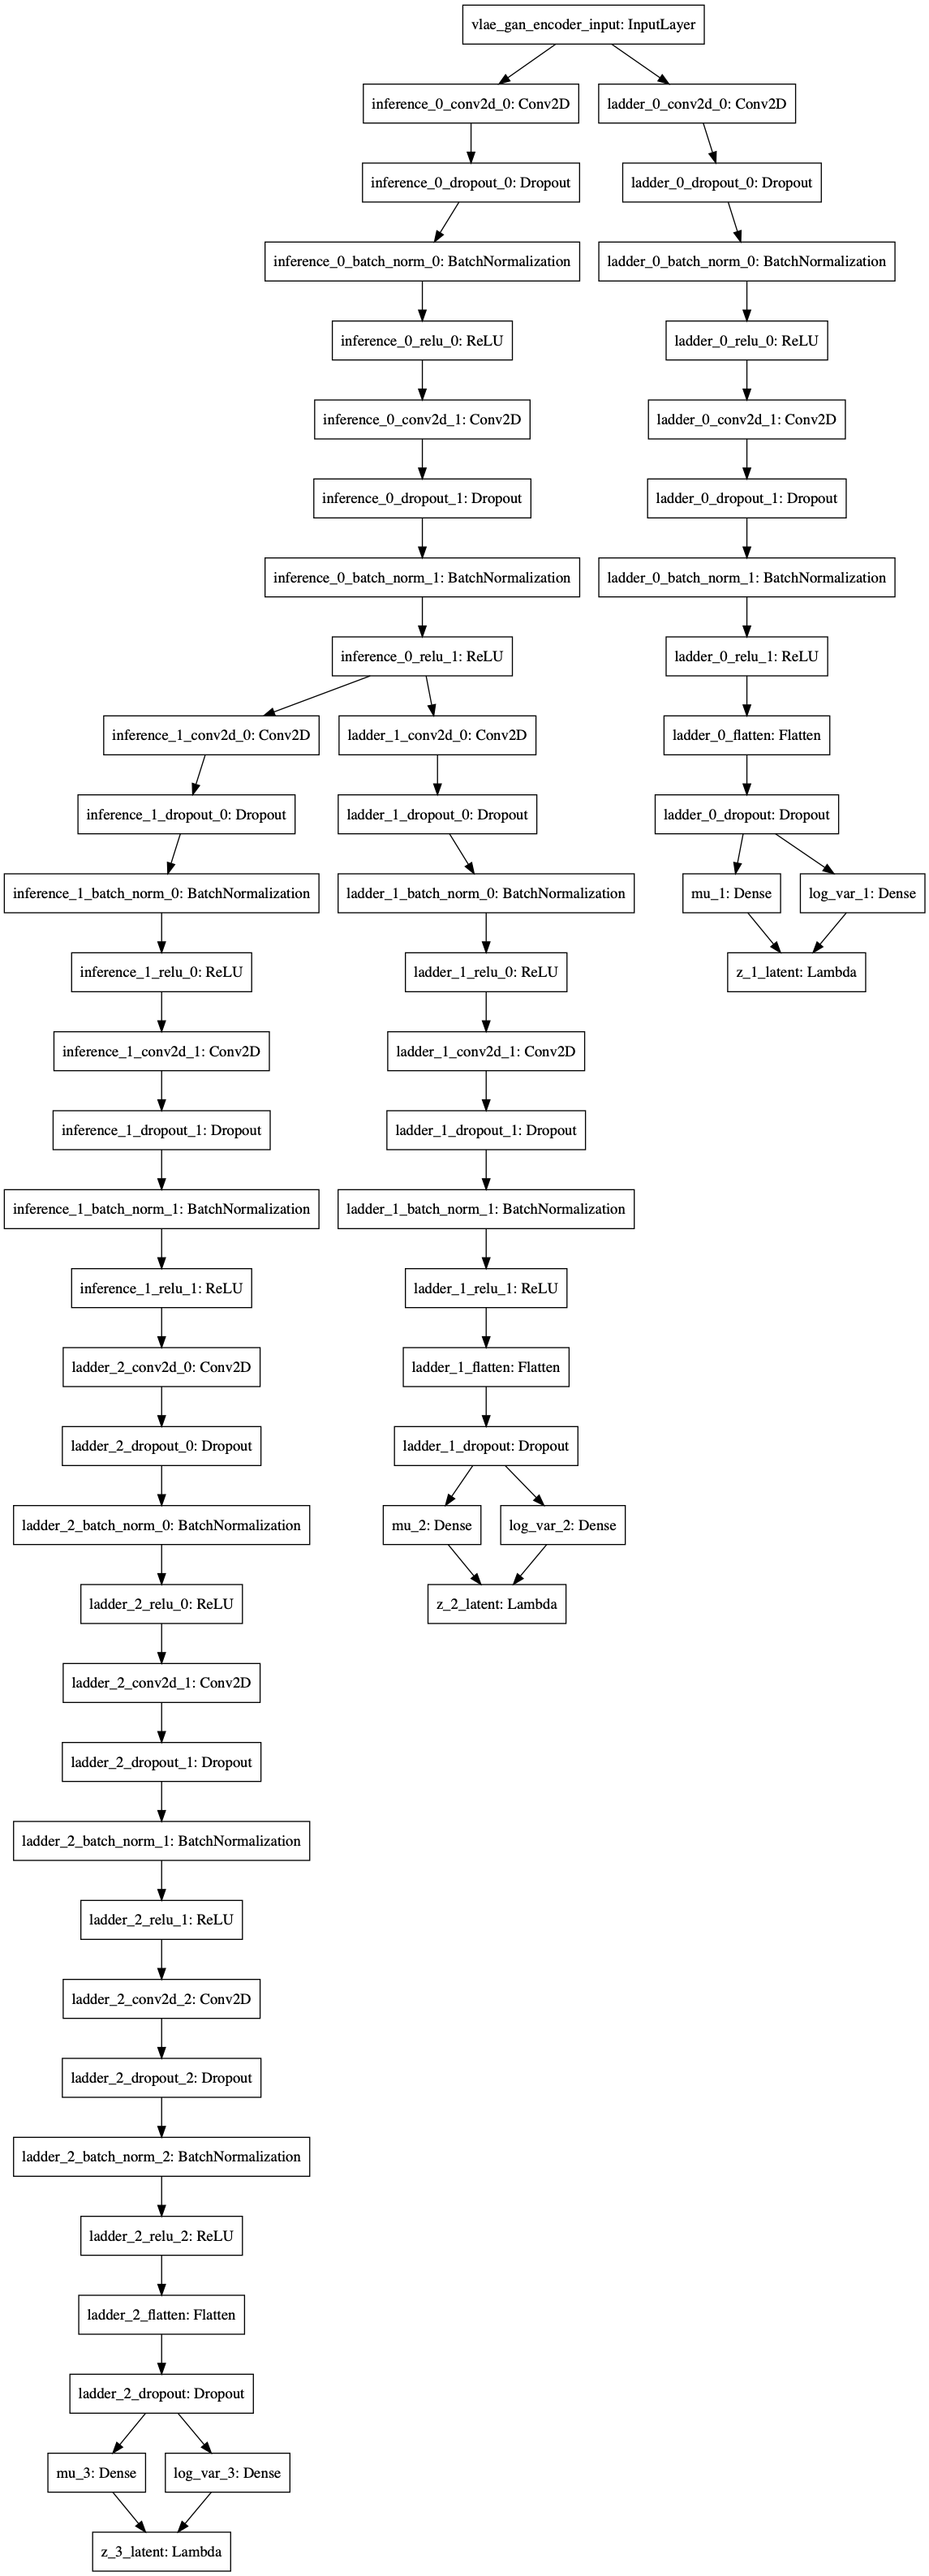
\includegraphics[width=\textwidth,height=.85\textheight,keepaspectratio]{images/vlae/encoder.png}
        \caption{Encoder}
        \label{subfig:vlae_encoder}
    \end{subfigure}%
    \begin{subfigure}{.5\textwidth}
        \centering
        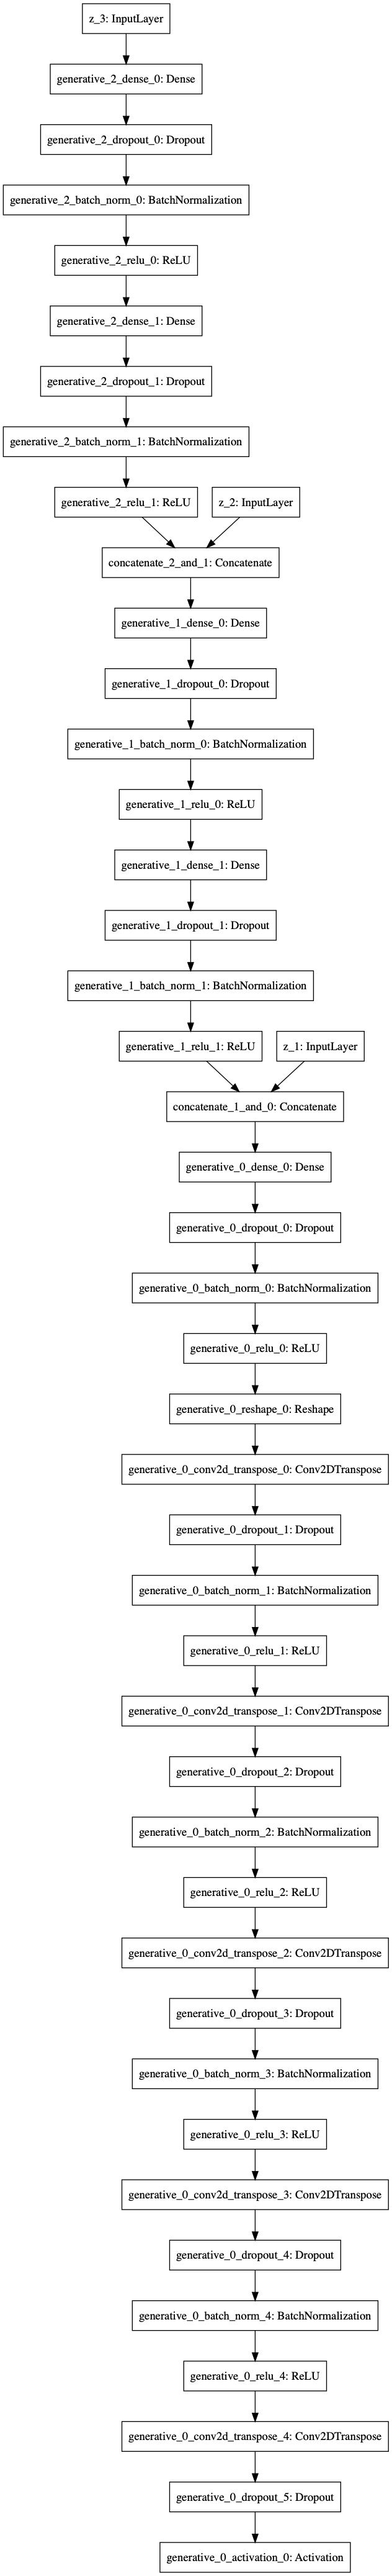
\includegraphics[width=\textwidth,height=.85\textheight,keepaspectratio]{images/vlae/decoder.png}
        \caption{Decoder}
        \label{subfig:vlae_decoder}
    \end{subfigure}
    \caption{\ac{VLAE} model structure}
    \label{fig:vlae_model_structure}
\end{figure}

Figure~\ref{fig:vlae_model_structure} shows the \ac{VLAE} model structure.
Like the \ac{VAE}, it consists of an encoder and a decoder.
The encoder has three latent spaces\footnote{\textit{z\_1\_latent}, \textit{z\_2\_latent}, and \textit{z\_3\_latent} in Figure~\ref{subfig:vlae_encoder}.}
A re-sampling according to Equation~\ref{eq:resampling_vae} is performed for each of the latent spaces.
Lower latent spaces are equipped with a less powerful encoder (e.g., \textit{z\_1\_latent} in Figure~\ref{subfig:vlae_encoder}), higher latent spaces with a more powerful encoder.
Again, the network is composed of multiple \say{Convolution, Activation, Batch-Normalization}-blocks.
The number of these blocks is variable and chosen depending on the dataset.
Batch-normalization can be omitted (default), the inner activation can be either ReLU (default) or LeakyReLU.
The convolutions use-zero padding, and encoder and decoder use stridden convolutions for downsampling.

The \ac{VAE} model implements the loss function from Equation~\ref{eq:elbo_error_term} but with a pre-factor for the reconstruction term.
The \ac{KL}-terms of different layers are totalized.

The decoder has three inputs, where the first input of the decoder\footnote{\textit{z\_3} in Figure~\ref{subfig:vlae_decoder}} receives input from the last output of the encoder\footnote{\textit{z\_3\_latent} in Figure~\ref{subfig:vlae_encoder}}.
The decoder uses blocks similar to the encoder but with transposed convolutions instead of regular convolutions.

In total, six \ac{VLAE}-models are used: \say{\textsc{Mnist}-\ac{VLAE}-factor-1}, \say{\textsc{Mnist}-\ac{VLAE}-factor-2}, \say{\textsc{Mnist}-\ac{VLAE}-factor-3} \say{dSprites-\ac{VLAE}}, \say{dSprites-\ac{VLAE}-dim2}, and \say{CelebA-\ac{VLAE}}.
The model structures can be found in Appendix~\ref{subseq:appendix_vlae_models}.

\paragraph{\textsc{Mnist}-\ac{VLAE}} The three \textsc{Mnist}-\ac{VLAE}s\footnote{\say{\textsc{Mnist}-\ac{VLAE}-factor-1}, \say{\textsc{Mnist}-\ac{VLAE}-factor-2}, \say{\textsc{Mnist}-\ac{VLAE}-factor-3}} use an input- and output-size of $28\times 28\times 1$.
The models are trained with the Adam optimizer on the \textsc{Mnist} training set with a batch size of 128 for 200 epochs.
The reconstruction loss factor is 10,000.
The latent spaces are two-dimensional.
The inner activation function is ReLU.
The models use no batch-normalization.
\textsc{Mnist}-\ac{VLAE}-factor-1 is the model with the original number of feature maps, for \textsc{Mnist}-\ac{VLAE}-factor-2 and \textsc{Mnist}-\ac{VLAE}-factor-3, the number of feature maps is reduced according to the factor.
\textsc{Mnist}-\ac{VLAE}-factor-1 is trained with a learning rate of 0.005.
\textsc{Mnist}-\ac{VLAE}-factor-2 and \textsc{Mnist}-\ac{VLAE}-factor-3 are trained with a learning rate of 0.001.

\paragraph{dSprites-\ac{VLAE}} dSprites-\ac{VLAE} uses an input- and output-size of $64\times 64\times 1$.
The model is trained with the Adam optimizer on a training set consisting of 90\% of the dSprites dataset with a batch size of 128 and a learning rate of 0.001 for 200 epochs.
The reconstruction loss factor is 10,000.
The latent spaces are four-dimensional.
The inner activation function is ReLU.

\paragraph{dSprites-\ac{VLAE}-dim2}
The dSprites-\ac{VLAE}-dim2 model is equivalent to dSprites-\ac{VLAE} but uses a two-dimensional latent space.

\paragraph{CelebA-\ac{VLAE}} CelebA-\ac{VLAE} uses an input- and output-size of $128\times 128\times 3$.
The model is trained with the Adam optimizer on a training set consisting of 90\% of the CelebA dataset with a batch size of 128, a learning rate of 0.001 with an additional learning rate decay of 0.01 for 200 epochs.
The reconstruction loss factor is 10,000.
The latent spaces are two-dimensional.
The inner activation function is ReLU.

\subsubsection{VAE-GAN Models}\label{subsubsec:vae_gan_models}

The \ac{VAE}-\ac{GAN}-model is similar to the \ac{VAE}-model.
However, it implements the \ac{VAE}-\ac{GAN} loss function (see Section~\ref{subsubsec:representation_learning}) instead of Equation~\ref{eq:elbo_error_term}.
Therefore, the \ac{VAE}-\ac{GAN} has an additional \textit{discriminator} network.
The feature loss compares inner activations in the discriminator of true and generated samples.
The discriminator loss signifies by how much the discriminator violates the \ac{GAN} training objective.
See Section~\ref{subsubsec:representation_learning} for more details.

For the encoder, the \ac{KL}-term is weighted ten-times more strongly than the feature loss.
The decoder weights the discriminator loss with factor 1 and the feature loss with factor 0.75.

In total, seven \ac{VAE}-\ac{GAN}-models are used: \say{\textsc{Mnist}-\ac{VAE}-\ac{GAN}}, \say{dSprites-\ac{VAE}-\ac{GAN}}, and \say{CelebA-\ac{VAE}-\ac{GAN}}.
The model structures can be found in Appendix~\ref{subseq:appendix_vae_gan_models}.

\paragraph{\textsc{Mnist}-\ac{VAE}-\ac{GAN}} \textsc{Mnist}-\ac{VAE}-\ac{GAN} uses an input- and output-size of $28\times 28\times 1$.
The model is trained with the Adam optimizer on the \textsc{Mnist} training set with a batch size of 128 and a learning rate of 0.0001 for 200 epochs.
The reconstruction loss factor is 10,000.
The latent space is two-dimensional.
The inner activation function is ReLU.

\paragraph{dSprites-\ac{VAE}-\ac{GAN}} dSprites-\ac{GAN} uses an input- and output-size of $64\times 64\times 1$.
The model is trained with the Adam optimizer on a training set consisting of 90\% of the dSprites dataset with a batch size of 128 and a learning rate of 0.0001 for 200 epochs.
The reconstruction loss factor is 10,000.
The latent space is ten-dimensional.
The inner activation function is ReLU.

\paragraph{CelebA-\ac{VAE}-\ac{GAN}} CelebA-\ac{VAE}-\ac{GAN} uses an input- and output-size of $128\times 128\times 3$.
The model is trained with the Adam optimizer on a training set consisting of 90\% of the CelebA dataset with a batch size of 128 and a learning rate of 0.001 with an additional learning rate decay of 0.02 for 200 epochs.
The reconstruction loss factor is 10,000.
The latent space is eight-dimensional.
The inner activation function is ReLU.

\subsubsection{VLAE-GAN Models}\label{subsubsec:vlae_gan_models}

The \ac{VLAE}-\ac{GAN}-model is comparable to the \ac{VAE}-\ac{GAN}-model in terms of the loss functions.
However, it uses the structure of the \ac{VLAE}-model and totalizes the three $KL$-losses from the different layers.

The model structures can be found in Appendix~\ref{subseq:appendix_vlae_gan_models}.

\paragraph{\textsc{Mnist}-\ac{VLAE}-\ac{GAN}} The three \textsc{Mnist}-\ac{VLAE}-\ac{GAN} uses an input- and output-size of $28\times 28\times 1$.
The model is trained with the Adam optimizer on the \textsc{Mnist} training set with a batch size of 128 and a learning rate of 0.0001 for 200 epochs.
The reconstruction loss factor is 10,000.
The latent spaces are two-dimensional.
The inner activation function is ReLU.
The model uses no batch-normalization.

\paragraph{dSprites-\ac{VLAE}-\ac{GAN}} dSprites-\ac{VLAE}-\ac{GAN} uses an input- and output-size of $64\times 64\times 1$.
The model is trained with the Adam optimizer on a training set consisting of 90\% of the dSprites dataset with a batch size of 128, a learning rate of 0.0001, and an additional learning rate decay of 0.01 for 200 epochs.
The reconstruction loss factor is 10,000.
The latent spaces are four-dimensional.
The inner activation function is ReLU.

\paragraph{CelebA-\ac{VLAE}-\ac{GAN}} CelebA-\ac{VLAE}-\ac{GAN} uses an input- and output-size of $128\times 128\times 3$.
The model is trained with the Adam optimizer on a training set consisting of 90\% of the CelebA dataset with a batch size of 128, a learning rate of 0.0001 with an additional learning rate decay of 0.01 for 200 epochs.
The reconstruction loss factor is 10,000.
The latent spaces are two-dimensional.
The inner activation function is ReLU.

\subsubsection{AlexNet Classifier}\label{subsubsec:alexnet_classifier}
The AlexNet Classifier resembles the architecture from \citet{krizhevsky2012imagenet}.
It uses dropout and a dropout rate of 0.3.
The model is trained with the Adam optimizer and a learning rate of 0.0001 using batch normalization and a batch size of 32 for ten epochs..
The model structure can be found in Appendix~\ref{subseq:appendix_alexnet_classifiers}.

\subsubsection{AlexNet-\ac{VAE}}\label{subsubsec:alexnet_vae}
The AlexNet-\ac{VAE} resembles the AlexNet classifier but uses a 2000-dimensional latent space with re-sampling (see Equation~\ref{eq:resampling_vae}).
For AlexNet-\ac{VAE}, no dropout is used.
The model is trained with the Adam optimizer and a learning rate of 0.0001 using batch normalization and a batch size of 32 for 100 epochs..
The model structure can be found in Appendix~\ref{subseq:appendix_alexnet_vae}.


    \section{Results}\label{sec:results}

    \subsection{Visual Features in Variational Autoencoders}\label{subsec:results_visual_features_in_variational_autoencoders}
    The following sections describe the results of the experiments on visual features in variational autoencoders.

    \begin{itemize}
        \item Results non-AlexNet-like-VAE on CelebA: especially layer 1 kernels
        \item Results AlexNet-like-VAE on ImageNet: especially layer 1 kernels
        \item Results AlexNet-like image classification CNN on ImageNet: especially layer 1 kernels
        \item Results AlexNet-like-VAE with frozen decoder from classification network
    \end{itemize}

    \subsubsection{AlexNet Image Classification}
    To make sure that the network structure of the \ac{VAE} is apt to generate Gabor wavelets, image classification was performed on ImageNet (see Figure~\ref{fig:alexnet} and Section~\ref{subsec:visual-features-variational-autoencoders} for the used network, see Section~\ref{ssec:imagenet} for ImageNet).
    As the accuracy was not of primary concern, the training was stopped during the tenth epoch (\textbf{If time: train all 100 epochs}), the top-1 training accuracy at this time was at 0.85.

    \begin{figure}
        \centering
        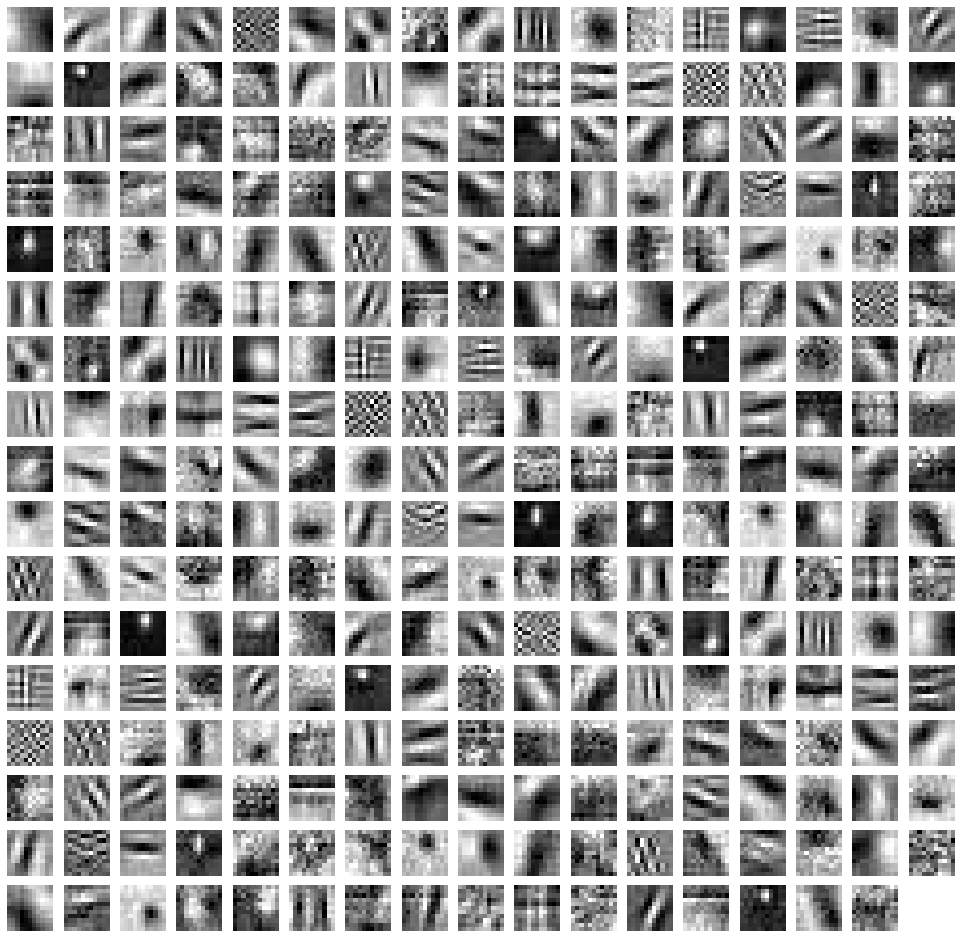
\includegraphics[width=0.9\textwidth]{images/alexnet_classification_l1_kernels.png}
        \caption[Image classification - Layer 1 Kernels]{Convolutional Kernels in the first layer of the image classification network. The filters are shown in their original size (11x11).}
        \label{fig:classification_layer1_kernels}
    \end{figure}

    Figure~\ref{fig:classification_layer1_kernels} shows all 256 convolutional kernels of the image classification network.
    It is easy to see that in many kernels, Gabor wavelet-like filters emerge.

    \subsection{Activity Correlation in \acp{VAE}}\label{subsec:results_activity-correlation-in-vaes}


    \section{Discussion}\label{sec:discussion}

    \subsection{Visual Features in Variational Autoencoders}\label{subsec:discussion_visual_features_in_variational_autoencoders}
    \begin{itemize}
        \item Reconstructions of AlexNet-VAE don't look natural at all, this might be because ImageNet, unlike CelebA, is not properly aligned and contains images from a large variety of classes.
        This might be another hint towards the assumption that \acp{VAE} are no suitable model for semantic representations
        \item How does it come that supervised models seem to be a good representation of \ac{IT} cortical representation~\citep{khaligh2014deep}? Maybe the brain learns in a ``supervised" manner in the sense that if you have never seen a horse, you need someone to tell you that that is a horse in order to make sense out of it.
        However, you might, at least, be able to recognize that it is an animal.
        Also, if someone tells you ``This is a horse.", you'll be able to recognize horses from different orientations and in different body positions without further training.
        This is quite different from how \acp{CNN} capture animals and is a strong hint to that supervised \acp{CNN} alone a no sufficient model for cortical IT representations.
    \end{itemize}


    \section{Conclusion}\label{sec:conclusion}

    \newpage
    \printbibliography

    \newpage
    \pagenumbering{Roman}
    \setcounter{page}{\thesavepage}
    \section*{Acronyms}
    \begin{acronym}[TDMA]
        \acro{VAE}{Variational Autoencoder}
        \acrodefplural{VAE}{Variational Autoencoders}
        \acro{CNN}{Convolutional Neural Network}
        \acrodefplural{CNN}{Convolutional Neural Networks}
        \acro{IT}{Inferior Temporal Cortex}
        \acro{ReLU}{Rectified Linear Unit}
        \acro{LeakyReLU}{Leaky Rectified Linear Unit}
        \acro{ILSVRC2017}{Large Scale Visual Recognition Challenge 2017}
    \end{acronym}
    \newpage
    \listoffigures
    \newpage
    \listoftables
    \newpage
    \section*{Erklärung}

Ich erkläre, dass das Thema dieser Arbeit nicht identisch ist mit dem Thema einer von mir bereits für eine andere Prüfung eingereichte Arbeit.\par
Ich erkläre weiterhin, dass ich die Arbeit nicht bereits an einer anderen Hochschule zur Erlangung eines akademischen Grades eingereicht habe.\par
\vspace{2cm}
Ich versichere, dass ich die Arbeit selbstständig verfasst und keine anderen als die angegebenen Quellen benutzt habe.
Die Stellen der Arbeit, die anderen Werken dem Wortlaut oder dem Sinn nach entnommen sind, habe ich unter Angabe der Quellen der Entlehnung kenntlich gemacht.
Dies gilt sinngemäß auch für gelieferte Zeichnungen, Skizzen, bildliche Darstellungen und dergleichen.

\vfill

\hspace{2cm} Ort, Datum \hfill Unterschrift \hspace{2cm}


\end{document}
